\chapter{Sparse Bayesian Learning}
So far, we have not addressed the central question: How do we solve the compressive sensing problem (\ref{eqn:CSproblem})?
Various deterministic approaches have been developed in recent years.
See \cite{pilikos2014} for an overview.

In the MPhil project, we will employ a probabilistic technique based on Sparse Bayesian Learning.
In particular, we will use the \emph{Relevance Vector Machine (RVM)} \cite{tipping2001,tipping2003} to reconstruct $\bs w$ from the measurements $\bs y$.
Following that, we obtain a reconstructed version of the desired signal $\bs x$ by pre-multiplying $\bs w$ by $\bs \Psi$ to obtain the desired signal.

The RVM is a \emph{regression} technique.
We model the relationship between $\bs y$ and $\bs x$ by
\begin{equation}
\label{eqn:rvmmodel}
y_i = \bs w^T \bs \psi(x_i) + \epsilon_i
\end{equation}
where $\psi(x_i)$ is the $i$th column of $\Psi$ and the $\epsilon_i$ are independent noise variables drawn from a zero-mean Gaussian distribution $\mathcal{N}(o,\sigma^2)$.

The model uses the available measurements $\{(x_1,y_1),\dots,(x_M,y_M)\}$ as training data to train the model in a Bayesian framework.
The result of training the RVM is a posterior distribution for the unknown vector of coefficients $\bs w$.
A special feature of the RVM is that the posterior mean $\bs \mu$ of $\bs w$ is often very sparse.

In order to reconstruct the image, we use the estimated posterior mean to ``predict'' what a pixel value $y^*$ should be at a location $x^*$ in which information was missing:
\begin{equation}
y^* = \bs w^T\bs\psi(x^*)
\end{equation}

\begin{figure}
\label{fig:lennareconstruction}
\center
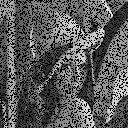
\includegraphics{0.png}
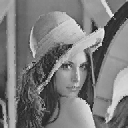
\includegraphics{3.png}
\caption{Corrupted signal $\bs y$ (left) and reconstructed signal $\hat{\bs x}$ (right) using a cascade of 3 RVMs with Haar basis functions (see \cite{pilikos2014}).}
\end{figure}

Apart from achieving sparse solutions, one further desirable feature of the RVM is that the model provides error bars for its predictions.
This is used in \cite{pilikos2014} to construct a multi-scale cascade of RVM estimations and achieve significant performance boosts.

An example of this can be seen in Figure \ref{fig:lennareconstruction}.

For details on the RVM and its implementation see \cite{pilikos2014,tipping2003,tipping2001}.

